% PAKETE UND DOKUMENTKONFIGURATION
\documentclass[11pt, a4paper]{article}

% Encoding für Umlaute
\usepackage[utf8]{inputenc}
\usepackage[T1]{fontenc}

% Silbentrennung
\usepackage[ngerman]{babel}

% erweiterte Matheumgebungen und Formelnummer mit Sectionnummer
\usepackage{amsmath}
\numberwithin{equation}{section}

% Braket Notation
\usepackage{braket}
\usepackage{isotope}
\usepackage{mhchem}

% zusätzliche mathematische Schriftarten
\usepackage{amsfonts}

% verschiedene mathematische Symbole
\usepackage{amssymb}

% Einheiten setzen z.B. \SI{10}{\kilo\gram\meter\per\second\squared}
% Fehler: \SI{10 +- 0,2e-4}{\metre}
\usepackage{siunitx}
\sisetup{
  output-decimal-marker={,},
  separate-uncertainty
}

% Einheitendefinitionen
\DeclareSIUnit{\skt}{Skt.}
\DeclareSIUnit{\gauss}{G}

% Operatordefinitionen
\DeclareMathOperator{\erf}{erf}

% Randbreiten
\usepackage[left=3.5cm,right=3.5cm,top=3cm,bottom=3cm,twoside]{geometry}

% Bilder einfügen
\usepackage{graphicx}

% Verweise innerhalb des Dokuments
\usepackage{hyperref}
\hypersetup{
	colorlinks = true,
	allcolors = {black}
}

% bessere Tabellenlayouts
\usepackage{booktabs}
\usepackage{multirow}
\usepackage{multicol}

% Seitenlayout (Kopfzeile)
\usepackage{fancyhdr}

% Float Barriers
\usepackage{placeins}

% Pakete für gedrehte Subfigures
\usepackage{caption}
\usepackage{subcaption}
\usepackage{rotating}

% Paket für textumflossene Abbildungen und Tabellen
\usepackage{wrapfig}

\usepackage{float}

% Caption-Setup
\captionsetup{font={small}}
\renewcommand{\thefigure}{\thesection.\arabic{figure}}
\renewcommand{\thesubfigure}{\alph{subfigure}}
\renewcommand{\thetable}{\thesection.\arabic{table}}
\renewcommand{\thesubtable}{\alph{subtable}}

% Manuelle Silbentrennung
\hyphenation{Re-so-na-tor Mo-den-ab-stand Re-so-na-tor-län-ge Spek-t-ro-me-ter}

% Tiefe des Inhaltsverzeichnisses (Level: 1 sections, 2 subsections,
% 3 subsubsections)
\setcounter{tocdepth}{3}

% FANCYHDR SETUP
\pagestyle{fancy}
\fancyhead[EL,OR]{\thepage}
\fancyhead[ER]{\leftmark}
\fancyhead[OL]{\rightmark}

\renewcommand{\sectionmark}[1]{
\markboth{\thesection{} #1}{\thesection{} #1}
}
\renewcommand{\subsectionmark}[1]{
\markright{\thesubsection{} #1}
}

\newcommand{\ptt}{Peak-to-Total-Verhältnis}

% DOKUMENTINFORMATIONEN
\title{P521 \\ Gamma-Spektroskopie mit Szintillations- und Halbleiterdetektoren}

\author{Christopher Deutsch\footnote{christopher.deutsch@uni-bonn.de} \and Christian Bespin\footnote{christian.bespin@uni-bonn.de}}

\date{\today}

\begin{document}

\begin{titlepage}

\maketitle

% DURCHFÜHRUNGSDATUM UND TUTOR
\begin{center}
\begin{tabular}{l r}
Durchführung: & 27./28. April 2015 \\
Gruppe: & $\alpha$ 6 \\
Tutor: & Christian Hammann
\end{tabular}
\end{center}

% ZUSAMMENFASSUNG
\begin{abstract}
\noindent

\end{abstract}

\end{titlepage}

% INHALTSVERZEICHNIS
\tableofcontents
% Neue Seite nach TOC
\newpage

% INHALT VERSUCHSPROTOKOLL

\section{Einführung}

\section{Theorie}

\subsection{Radioaktiver Zerfall}

\subsubsection{Quellen radioaktiver Strahlung}
\label{sssec:quellen_radioaktivität}
Man kategorisiert Quellen radioaktiver Strahlung meistens in \textbf{natürliche Radioaktivität} und \textbf{künstliche Radioaktivität}.
Zu ersterem werden vor allem radioaktive Nuklide gezählt, die bereits seit Entstehung der Erde existieren und heute noch nachweisbar sind (primordiale Nuklide).
Weiterhin werden Nuklide, die bei Zerfällen dieser entstehen sowie kosmische Strahlung der natürlichen Radioaktivität zugeordnet.
Künstliche Radioakivität entsteht gezielt oder als Abfallprodukt bei gesteuerten Prozessen wie der Kernspaltung zur Energiegewinnung oder für medizinischen und technische Anwendungen.

\subsubsection{Zerfallsreihen}

Als Zerfallsreihe bezeichnet man eine Kette radioaktiver Zerfälle, bei denen das aus dem zerfallenden Nuklid entstehende Tochternuklid weiter über radioaktiven Zerfall zerfällt.
Von besonderem Interesse sind die natürlichen Zerfallsreihen, die diese Kette radioaktiver Zerfälle für die primordialen Nuklide (s. \ref{sssec:quellen_radioaktivität}) beschreiben.
Es werden hier nur einige der Nuklide aufgeführt, da die Reihen recht lang sind und sich zwischendurch auch verzweigen können (dies geschieht, wenn ein Nuklid in mehrere andere zerfallen kann).
\begin{align*}
	&\isotope[244]{Pu}\to\dots\to\isotope[232]{Th}\to\dots\to\isotope[228]{Th}\to\dots\to\isotope[208]{Pb} &\qquad\text{(Thoriumreihe)}\\
	&\isotope[238]{U}\to\dots\to\isotope[226]{Ra}\to\dots\to\isotope[214]{Pb}\to\dots\to\isotope[206]{Pb} &\qquad\text{(Uran-Radium-Reihe)}\\
	&\isotope[235]{U}\to\dots\to\isotope[227]{Ac}\to\dots\to\isotope[211]{Pb}\to\dots\to\isotope[207]{Pb} &\qquad\text{(Uran-Actinium-Reihe)}
\end{align*}
Die als Thoriumreihe bezeichnete Zerfallsreihe beginnt zwar mit einem Pulloniumnuklid, ist jedoch nach dem am häufigsten auftretenden Element Thorium benannt.
Es existiert darüber hinaus noch eine Neptunium-Reihe ($\isotope[237]{Np}\to\isotope[205]{Tl}$), diese zählt allerdings nicht mehr zu den natürlichen Zerfallsreihen, da das bei Entstehung der Erde vorhandene Neptunium mittlerweile komplett zerfallen ist.
Sie kann nur noch auf künstlichem Weg erzeugt werden, da \isotope[237]{Np} ein Tochternuklid von in Kernreaktoren erzeugten Nukliden ist.

\subsubsection{$\gamma$-Strahlung}

In diesem Versuch wird der atomare Zerfallsprozess mit $\gamma$-Strahlung betrachtet.
Sie entsteht wenn ein energetisch angeregter Atomkern in einen energetisch weniger angeregten Zustand übergeht.
Die dabei frei werdende Energie wird in Form von hochenergetischen Photonen, s.g. Gamma-Quanten ausgesendet, deren Energiebereich von wenigen hundert \si{\kilo\electronvolt} bis zu mehreren \si{\mega\electronvolt} reicht.

\subsection{Wechselwirkung von $\gamma$-Quanten mit Materie}

Die Wechselwirkung von $\gamma$-Quanten mit Materie kann hauptsächlich auf drei verschiedene Arten erfolgen.
Dabei ist vor allem ihr jeweiliger Wirkungsquerschnitt von Interesse, der angibt, wie die Wechselwirkung der hochenergetischen Photonen von der Energie und Ordnungszahl abhängt.
Ausgehend davon kann beispielsweise festgestellt werden, auf welchen Energiebereichen welche Form der Wechselwirkung dominiert.

\subsubsection{Photoeffekt}
Im Bereich niedriger Energie tritt vor allem der Photoeffekt auf.
Dieser beschreibt die Absoprtion eines Gamma-Quants durch ein atomisches Elektron und kann aufgrund der Impulserhaltung nur im Atom stattfinden.
Bei Einstrahlung eines Photons wird dieses absorbiert und ein Elektron aus dem Atom herausgelöst, dessen Energie der Enerie des Photons entspricht abzüglich der Bindungsenergie.
\begin{align*}
E_\mathrm{e^{-}} = h \nu - E_\mathrm{Bind.}
\end{align*}
Der Wirkungsquerschnitt ist gegeben durch:
\begin{align*}
	\sigma_\mathrm{Photo.} \propto
	\begin{cases}
		Z^5 E_\gamma^{-\frac{7}{2}} & E_\gamma < m_\mathrm{e} c^2 \\
		Z^5 E_\gamma^{-1} & E_\gamma > m_\mathrm{e} c^2
	\end{cases}
\end{align*}
Quelle: Siegbahn
\begin{figure}[h]
	\centering
	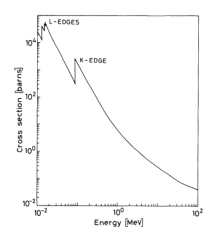
\includegraphics{./figures/photoeffekt.png}
	\caption{Wirkungsquerschnitt für den Photoeffekt an Blei. QUELLE William R. Leo}
	\label{fig:photoeffekt}
\end{figure}

\subsubsection{Compton-Effekt}
Der Compton-Effekt beschreibt die Streuung von Photonen an freien Elektronen.
Allerdings können Elektronen im Fall $E_\gamma \gg E_\mathrm{Bind. e^{-}}$ auch in Materie als frei betrachtet werden.
Die Streuung beschreibt einen winkelabhängigen Energieübertrag vom Photon auf das Elektron, wobei der Streuwinkel $\theta$ des Photons relativ zur einfallenden Flugrichtung angegeben wird.

(BILD mit Winkeln undso)

\begin{align}
	\frac{E_\gamma^\prime}{E_\gamma} &= \frac{1}{1 + \frac{h \nu}{m_\mathrm{e} c^2} (1-\cos\theta)} \\
	\Delta \lambda &= \lambda_\mathrm{c} (1 - \cos\theta) \\
	\lambda_\mathrm{c} &= \frac{h}{m_\mathrm{e} c}
\end{align}
Wirkungsquerschnitt gegeben durch Klein-Nishina:
\begin{align}
	\sigma_\mathrm{c} \propto \frac{Z}{E_\gamma}
\end{align}

Compton-Kante...

Kein Energietransfer:\\
Thomson-Streuung: Compton im klassischen Limit\\
Rayleigh-Streuung: Streuung am ganzen Atom\\


\subsubsection{Paarbildung}
\begin{align}
	\gamma \rightarrow \mathrm{e}^{+} + \mathrm{e}^{-}\\
	E_\gamma \geq 2 m_\mathrm{e} c^2
\end{align}

\begin{align}
	\sigma_\mathrm{Paar} \propto Z^2 \ln E_\gamma
\end{align}

\subsubsection{Summe aller Effekte}

Bildah

\subsection{Szintillatoren, Halbleiterdetektor, Photomulti etc.}

\subsubsection{Detektor Charakteristiken}
Output des Detektors ein Strompuls und die Energie des detektierten Teilchens ist proportional zu der Ladung des Pulses.
Ist die Pulsform von Teilchen verschiedener Energien immer gleich, so ist dies gleichbedeutend zu der Höhe des Pulses.\\
\\
Energieauflösung: Linien haben Gaußform. Weite der Linie verursacht durch Fluktuationen in der Anzahl der Ionisationen/Anregungen(Poissonverteilt) (statistischer Prozess: $\mathcal{R} \propto 1 / \sqrt{N}$ mit der Anzahl der Ionisationen bei gegebener Energie $N$. Zentraler Grenzwertsatz: $\sigma_x^2 / \braket{X} \propto 1 / \sqrt{N}$, wobei X eine Summe von N Zufallsvariablen ist.).
Auflösung (FWHM):
\begin{align}
	\text{Resolution} = \frac{\Delta E}{E}
\end{align}
Auflösung ist eine Funktion der Energie! Generell ist die Anzahl der Ionisationen proportional zur Energie des einfallenden Teilchens. Damit skaliert die Auflösung ebenfalls wie:
\begin{align}
	\mathcal{R} \propto \frac{1}{\sqrt{E_\gamma}}
\end{align}
Neben der intrinsischen Unschärfe des Detektors kommt noch Unschärfe der verwendeten Elektron, welche sich quadratisch addiert:
\begin{align}
	\Delta E^2 = \Delta E_\mathrm{Detektor}^2 + \Delta E_\mathrm{Elektronik}^2
\end{align}
\\
Detektoreffizienz: Unterscheidung zwischen absoluter und intrinsischer Effizienz.\\
Absolute (totale) Effizienz:
\begin{align}
	\mathcal{E}_\mathrm{tot} = \frac{\text{events registered}}{\text{events emitted by source}}
\end{align}
(Peakeffizienz: events registered $\rightarrow$ Ereignisse im Photopeak) 
Ist abhängig von der Detektorgeometrie und der Wahrscheinlichkeit einer Interaktion mit dem Detektor.\\
\\
Intrinsische Effizienz:
\begin{align}
	\mathcal{E}_\mathrm{int} = \frac{\text{events registered}}{\text{events impinging on detector}}
\end{align}
Mit der absoluten Peakeffizienz scheint die intrinsische Effizienz aus Leo gemeint zu sein.
\begin{align}
	\mathcal{E}_\mathrm{int} = \frac{N_\mathrm{Photo.}}{A \cdot T \cdot \frac{\pi r^2}{4\pi \, d^2}}
\end{align}
Der geometrische Faktor im Nenner geht von einer Punktquelle (Aktivität $A$) in hohem Abstand vom Detektor $d$ aus. Messzeit $T$, Detektorradius $r$.

\subsubsection{Szintillatoren}
Szintillator: Körper dessen Moleküle beim Durchgang von energiereichen Photonen angeregt werden und folglich Licht (meist im UV-Bereich) emittieren. In Kombination mit Photomulti geeignete Detektoren.\\
\\
Über einer Mindestenergie verhalten sich Szintillatoren linear (Lichtenerzeugung - Energie des Photons)
\\
Besteht aus Kristall mit Aktivator-Zentren (Dotierung)\\
Einfallendes Photon löst $\mathrm{e}^{-}$-Kaskade aus bis Energie klein genug ist um wieder in Atomen gefangen zu werden $\rightarrow$ Photonenemission\\
Kristall selber ist nicht transparent für diese Photonen. Dotierung erzeugt neue Energieniveaus, über welche Photonen erzeugt werden für die das Material transparent ist.\\
Oft mit Thallium aktivierte NaI-Kristalle wegen der hohen Ordnungszahl von Jod(Iod).\\
\\
Exciton: Unreinheiten im Kristall verursachen ein Exciton-Band unter dem Leitungsband. Ein einfallendes Photon erzeugt nur ein Exciton (e-Loch-Paar) im Exciton-Band/Valenzband, welches frei im Kristall beweglich ist. Trifft dieses Exciton auf eine Verunreinigung (Thallium) kann dieses durch das Loch des Excitons ionisiert werden und das Exciton über ein lokales Energieniveau aufgrund der Verunreinigung abgeregt werden (unter Emission von Photonen).\\
\\
Für die Detektion von Photonen sind hohe Ordnungszahlen $Z$ wünscheswert (vgl. Wirkungsquerschnitt Photoeffekt im vergleich zu Compton)

\subsubsection{Halbleiterdetektor}
Analog zum Gas-Ionisationsdetektor nur dass Elektronen-Loch Paare statt Elektron-Ion-Paare erzeugt werden.
Vorteil: Erzeugung von e-Loch-Paar benötigt weniger Energie (Bandlücke); dadurch mehr Paare.\\
\\
Höhere Dichte höhere stopping-power (mehr Energiedeposition).\\
\\
Kompakt und hohe response time.\\
\\
Außer Silizium benötigen sie Kühlung da thermische e-Loch-Paare erzeugt werden können. Größter Faktor aber trotzdem Oberflächenströme, daher wird ein gut verkapselter Detektor benötigt.\\
\\
Rekombination in Halbleitern ist selten, da Loch und Elektron Impuls und Energieerhaltung erfüllen müssen(Lebenszeiten Größenordnung Sekunde).
Rekombinationszentren: Verunreinigung sorgen für weitere Energieniveaus zwischen Valenz und Leitungsband, welche ein Elektron einfangen können. Folge: a) Das Elektron geht wieder in das Leitungsband. b) Nach einer Zeit trifft auf die Verunreinigung ein Loch, welches mit dem gefangenen Elektron annhiliert.
Es folgt das Halbleiterdetektoren sehr reine Kristalle benötigt, da die Ladung an den Kathoden eingefangen werden soll.\\
\\
Trapping: Verunreinheiten die nur einen Typ von Ladungsträger (Elektron, Loch) einfangen können und diese für eine gewisse Zeit halten und danach wieder freigeben. Negativer Einfluss auf die Ladungssammlung.
Ähnlicher Effekt durch Gitterdefekte.\\
\\
PN-Übergang in reverse Bias. In der Verarmungszone werden Elektron-Loch-Paare erzeugt (durch ionisierende Strahlung) die als Strompuls gemessen werden können. Reverse Bias: 1) Verarmungszone ist größer dadurch wird mehr Strahlung detektiert 2) Feld in der Verarmungszone ist größer und begünstigt die Ladungssammlung. An den Metallkontakten muss der Halbleiter stark dotiert sein um einen ohmschen Übergang zu erlauben. (sonst wirkt er wie eine Diode)\\
\\
Energie für e-Loch-Bildung:
\begin{align}
	E_\mathrm{Ge} = \SI{2.96}{eV} \quad \text{@ 77 K}
\end{align}
Mehr als Bandlücke da ein Teil der Energie in Anregungen des Gitter übergeht.
Cite William R. Leo\\
Im Vergleich zur Photoelektronenbildung in Szintillatoren zwei Größenordnung höhere e-Loch-Bildung und damit bessere Energieauflösung.\\
\\
Aufgrund der hohen Ordnungszahl von Germanium ist der Photowirkungsquerschnitt 60 mal größer als der von Silizium.\\
Vergleich von Germanium und NaI-Detektor im Leo Fig. 10{.}19.

\begin{figure}[h]
	\centering
	% GNUPLOT: LaTeX picture with Postscript
\begingroup
  \makeatletter
  \providecommand\color[2][]{%
    \GenericError{(gnuplot) \space\space\space\@spaces}{%
      Package color not loaded in conjunction with
      terminal option `colourtext'%
    }{See the gnuplot documentation for explanation.%
    }{Either use 'blacktext' in gnuplot or load the package
      color.sty in LaTeX.}%
    \renewcommand\color[2][]{}%
  }%
  \providecommand\includegraphics[2][]{%
    \GenericError{(gnuplot) \space\space\space\@spaces}{%
      Package graphicx or graphics not loaded%
    }{See the gnuplot documentation for explanation.%
    }{The gnuplot epslatex terminal needs graphicx.sty or graphics.sty.}%
    \renewcommand\includegraphics[2][]{}%
  }%
  \providecommand\rotatebox[2]{#2}%
  \@ifundefined{ifGPcolor}{%
    \newif\ifGPcolor
    \GPcolortrue
  }{}%
  \@ifundefined{ifGPblacktext}{%
    \newif\ifGPblacktext
    \GPblacktexttrue
  }{}%
  % define a \g@addto@macro without @ in the name:
  \let\gplgaddtomacro\g@addto@macro
  % define empty templates for all commands taking text:
  \gdef\gplbacktext{}%
  \gdef\gplfronttext{}%
  \makeatother
  \ifGPblacktext
    % no textcolor at all
    \def\colorrgb#1{}%
    \def\colorgray#1{}%
  \else
    % gray or color?
    \ifGPcolor
      \def\colorrgb#1{\color[rgb]{#1}}%
      \def\colorgray#1{\color[gray]{#1}}%
      \expandafter\def\csname LTw\endcsname{\color{white}}%
      \expandafter\def\csname LTb\endcsname{\color{black}}%
      \expandafter\def\csname LTa\endcsname{\color{black}}%
      \expandafter\def\csname LT0\endcsname{\color[rgb]{1,0,0}}%
      \expandafter\def\csname LT1\endcsname{\color[rgb]{0,1,0}}%
      \expandafter\def\csname LT2\endcsname{\color[rgb]{0,0,1}}%
      \expandafter\def\csname LT3\endcsname{\color[rgb]{1,0,1}}%
      \expandafter\def\csname LT4\endcsname{\color[rgb]{0,1,1}}%
      \expandafter\def\csname LT5\endcsname{\color[rgb]{1,1,0}}%
      \expandafter\def\csname LT6\endcsname{\color[rgb]{0,0,0}}%
      \expandafter\def\csname LT7\endcsname{\color[rgb]{1,0.3,0}}%
      \expandafter\def\csname LT8\endcsname{\color[rgb]{0.5,0.5,0.5}}%
    \else
      % gray
      \def\colorrgb#1{\color{black}}%
      \def\colorgray#1{\color[gray]{#1}}%
      \expandafter\def\csname LTw\endcsname{\color{white}}%
      \expandafter\def\csname LTb\endcsname{\color{black}}%
      \expandafter\def\csname LTa\endcsname{\color{black}}%
      \expandafter\def\csname LT0\endcsname{\color{black}}%
      \expandafter\def\csname LT1\endcsname{\color{black}}%
      \expandafter\def\csname LT2\endcsname{\color{black}}%
      \expandafter\def\csname LT3\endcsname{\color{black}}%
      \expandafter\def\csname LT4\endcsname{\color{black}}%
      \expandafter\def\csname LT5\endcsname{\color{black}}%
      \expandafter\def\csname LT6\endcsname{\color{black}}%
      \expandafter\def\csname LT7\endcsname{\color{black}}%
      \expandafter\def\csname LT8\endcsname{\color{black}}%
    \fi
  \fi
    \setlength{\unitlength}{0.0500bp}%
    \ifx\gptboxheight\undefined%
      \newlength{\gptboxheight}%
      \newlength{\gptboxwidth}%
      \newsavebox{\gptboxtext}%
    \fi%
    \setlength{\fboxrule}{0.5pt}%
    \setlength{\fboxsep}{1pt}%
\begin{picture}(7200.00,5040.00)%
    \gplgaddtomacro\gplbacktext{%
      \csname LTb\endcsname%
      \put(946,704){\makebox(0,0)[r]{\strut{}$0$}}%
      \csname LTb\endcsname%
      \put(946,1286){\makebox(0,0)[r]{\strut{}$200$}}%
      \csname LTb\endcsname%
      \put(946,1867){\makebox(0,0)[r]{\strut{}$400$}}%
      \csname LTb\endcsname%
      \put(946,2449){\makebox(0,0)[r]{\strut{}$600$}}%
      \csname LTb\endcsname%
      \put(946,3030){\makebox(0,0)[r]{\strut{}$800$}}%
      \csname LTb\endcsname%
      \put(946,3612){\makebox(0,0)[r]{\strut{}$1000$}}%
      \csname LTb\endcsname%
      \put(946,4193){\makebox(0,0)[r]{\strut{}$1200$}}%
      \csname LTb\endcsname%
      \put(946,4775){\makebox(0,0)[r]{\strut{}$1400$}}%
      \csname LTb\endcsname%
      \put(1078,484){\makebox(0,0){\strut{}$0$}}%
      \csname LTb\endcsname%
      \put(2223,484){\makebox(0,0){\strut{}$1000$}}%
      \csname LTb\endcsname%
      \put(3368,484){\makebox(0,0){\strut{}$2000$}}%
      \csname LTb\endcsname%
      \put(4513,484){\makebox(0,0){\strut{}$3000$}}%
      \csname LTb\endcsname%
      \put(5658,484){\makebox(0,0){\strut{}$4000$}}%
      \csname LTb\endcsname%
      \put(6803,484){\makebox(0,0){\strut{}$5000$}}%
    }%
    \gplgaddtomacro\gplfronttext{%
      \csname LTb\endcsname%
      \put(176,2739){\rotatebox{-270}{\makebox(0,0){\strut{}Ereignisse $N$}}}%
      \put(3940,154){\makebox(0,0){\strut{}Kanal $n$}}%
      \csname LTb\endcsname%
      \put(5816,4602){\makebox(0,0)[r]{\strut{}Messwerte}}%
    }%
    \gplbacktext
    \put(0,0){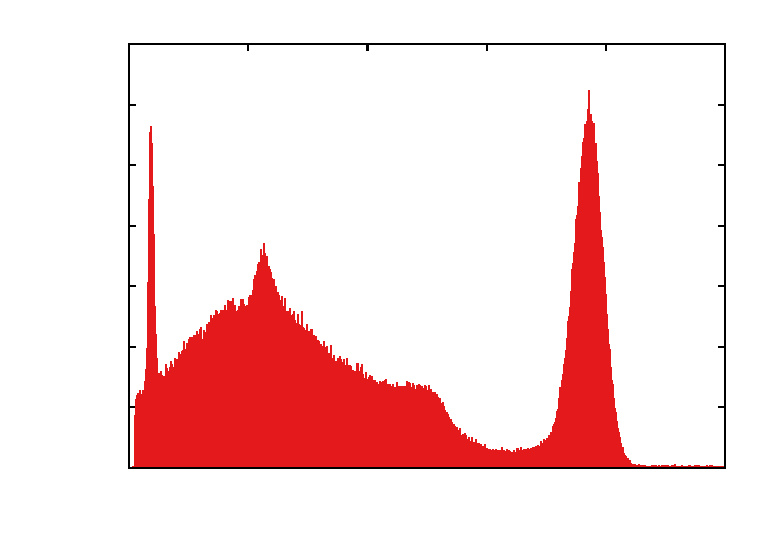
\includegraphics{./plots/szintillator/caesium}}%
    \gplfronttext
  \end{picture}%
\endgroup

	\caption{Cääääääsium szinti}
	\label{fig:caesium_spektrum}
\end{figure}

\begin{figure}[h]
	\centering
	% GNUPLOT: LaTeX picture with Postscript
\begingroup
  \makeatletter
  \providecommand\color[2][]{%
    \GenericError{(gnuplot) \space\space\space\@spaces}{%
      Package color not loaded in conjunction with
      terminal option `colourtext'%
    }{See the gnuplot documentation for explanation.%
    }{Either use 'blacktext' in gnuplot or load the package
      color.sty in LaTeX.}%
    \renewcommand\color[2][]{}%
  }%
  \providecommand\includegraphics[2][]{%
    \GenericError{(gnuplot) \space\space\space\@spaces}{%
      Package graphicx or graphics not loaded%
    }{See the gnuplot documentation for explanation.%
    }{The gnuplot epslatex terminal needs graphicx.sty or graphics.sty.}%
    \renewcommand\includegraphics[2][]{}%
  }%
  \providecommand\rotatebox[2]{#2}%
  \@ifundefined{ifGPcolor}{%
    \newif\ifGPcolor
    \GPcolortrue
  }{}%
  \@ifundefined{ifGPblacktext}{%
    \newif\ifGPblacktext
    \GPblacktexttrue
  }{}%
  % define a \g@addto@macro without @ in the name:
  \let\gplgaddtomacro\g@addto@macro
  % define empty templates for all commands taking text:
  \gdef\gplbacktext{}%
  \gdef\gplfronttext{}%
  \makeatother
  \ifGPblacktext
    % no textcolor at all
    \def\colorrgb#1{}%
    \def\colorgray#1{}%
  \else
    % gray or color?
    \ifGPcolor
      \def\colorrgb#1{\color[rgb]{#1}}%
      \def\colorgray#1{\color[gray]{#1}}%
      \expandafter\def\csname LTw\endcsname{\color{white}}%
      \expandafter\def\csname LTb\endcsname{\color{black}}%
      \expandafter\def\csname LTa\endcsname{\color{black}}%
      \expandafter\def\csname LT0\endcsname{\color[rgb]{1,0,0}}%
      \expandafter\def\csname LT1\endcsname{\color[rgb]{0,1,0}}%
      \expandafter\def\csname LT2\endcsname{\color[rgb]{0,0,1}}%
      \expandafter\def\csname LT3\endcsname{\color[rgb]{1,0,1}}%
      \expandafter\def\csname LT4\endcsname{\color[rgb]{0,1,1}}%
      \expandafter\def\csname LT5\endcsname{\color[rgb]{1,1,0}}%
      \expandafter\def\csname LT6\endcsname{\color[rgb]{0,0,0}}%
      \expandafter\def\csname LT7\endcsname{\color[rgb]{1,0.3,0}}%
      \expandafter\def\csname LT8\endcsname{\color[rgb]{0.5,0.5,0.5}}%
    \else
      % gray
      \def\colorrgb#1{\color{black}}%
      \def\colorgray#1{\color[gray]{#1}}%
      \expandafter\def\csname LTw\endcsname{\color{white}}%
      \expandafter\def\csname LTb\endcsname{\color{black}}%
      \expandafter\def\csname LTa\endcsname{\color{black}}%
      \expandafter\def\csname LT0\endcsname{\color{black}}%
      \expandafter\def\csname LT1\endcsname{\color{black}}%
      \expandafter\def\csname LT2\endcsname{\color{black}}%
      \expandafter\def\csname LT3\endcsname{\color{black}}%
      \expandafter\def\csname LT4\endcsname{\color{black}}%
      \expandafter\def\csname LT5\endcsname{\color{black}}%
      \expandafter\def\csname LT6\endcsname{\color{black}}%
      \expandafter\def\csname LT7\endcsname{\color{black}}%
      \expandafter\def\csname LT8\endcsname{\color{black}}%
    \fi
  \fi
    \setlength{\unitlength}{0.0500bp}%
    \ifx\gptboxheight\undefined%
      \newlength{\gptboxheight}%
      \newlength{\gptboxwidth}%
      \newsavebox{\gptboxtext}%
    \fi%
    \setlength{\fboxrule}{0.5pt}%
    \setlength{\fboxsep}{1pt}%
\begin{picture}(7200.00,5040.00)%
    \gplgaddtomacro\gplbacktext{%
      \csname LTb\endcsname%
      \put(1078,704){\makebox(0,0)[r]{\strut{}$0$}}%
      \csname LTb\endcsname%
      \put(1078,1383){\makebox(0,0)[r]{\strut{}$2000$}}%
      \csname LTb\endcsname%
      \put(1078,2061){\makebox(0,0)[r]{\strut{}$4000$}}%
      \csname LTb\endcsname%
      \put(1078,2740){\makebox(0,0)[r]{\strut{}$6000$}}%
      \csname LTb\endcsname%
      \put(1078,3418){\makebox(0,0)[r]{\strut{}$8000$}}%
      \csname LTb\endcsname%
      \put(1078,4097){\makebox(0,0)[r]{\strut{}$10000$}}%
      \csname LTb\endcsname%
      \put(1078,4775){\makebox(0,0)[r]{\strut{}$12000$}}%
      \csname LTb\endcsname%
      \put(1210,484){\makebox(0,0){\strut{}$0$}}%
      \csname LTb\endcsname%
      \put(1831,484){\makebox(0,0){\strut{}$1000$}}%
      \csname LTb\endcsname%
      \put(2453,484){\makebox(0,0){\strut{}$2000$}}%
      \csname LTb\endcsname%
      \put(3074,484){\makebox(0,0){\strut{}$3000$}}%
      \csname LTb\endcsname%
      \put(3696,484){\makebox(0,0){\strut{}$4000$}}%
      \csname LTb\endcsname%
      \put(4317,484){\makebox(0,0){\strut{}$5000$}}%
      \csname LTb\endcsname%
      \put(4939,484){\makebox(0,0){\strut{}$6000$}}%
      \csname LTb\endcsname%
      \put(5560,484){\makebox(0,0){\strut{}$7000$}}%
      \csname LTb\endcsname%
      \put(6182,484){\makebox(0,0){\strut{}$8000$}}%
      \csname LTb\endcsname%
      \put(6803,484){\makebox(0,0){\strut{}$9000$}}%
    }%
    \gplgaddtomacro\gplfronttext{%
      \csname LTb\endcsname%
      \put(176,2739){\rotatebox{-270}{\makebox(0,0){\strut{}Ereignisse $$}}}%
      \put(4006,154){\makebox(0,0){\strut{}Kanal $n$}}%
      \csname LTb\endcsname%
      \put(2530,4602){\makebox(0,0)[r]{\strut{}Messwerte}}%
    }%
    \gplbacktext
    \put(0,0){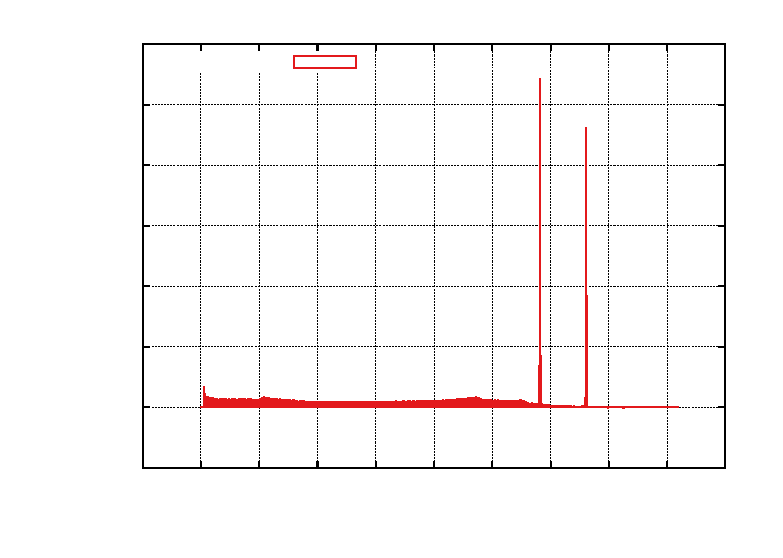
\includegraphics{./plots/halbleiter/cobalt}}%
    \gplfronttext
  \end{picture}%
\endgroup

	\caption{Cooooobalt szinti}
	\label{fig:cobalt_spektrum}
\end{figure}

\begin{figure}[h]
	\centering
	% GNUPLOT: LaTeX picture with Postscript
\begingroup
  \makeatletter
  \providecommand\color[2][]{%
    \GenericError{(gnuplot) \space\space\space\@spaces}{%
      Package color not loaded in conjunction with
      terminal option `colourtext'%
    }{See the gnuplot documentation for explanation.%
    }{Either use 'blacktext' in gnuplot or load the package
      color.sty in LaTeX.}%
    \renewcommand\color[2][]{}%
  }%
  \providecommand\includegraphics[2][]{%
    \GenericError{(gnuplot) \space\space\space\@spaces}{%
      Package graphicx or graphics not loaded%
    }{See the gnuplot documentation for explanation.%
    }{The gnuplot epslatex terminal needs graphicx.sty or graphics.sty.}%
    \renewcommand\includegraphics[2][]{}%
  }%
  \providecommand\rotatebox[2]{#2}%
  \@ifundefined{ifGPcolor}{%
    \newif\ifGPcolor
    \GPcolortrue
  }{}%
  \@ifundefined{ifGPblacktext}{%
    \newif\ifGPblacktext
    \GPblacktexttrue
  }{}%
  % define a \g@addto@macro without @ in the name:
  \let\gplgaddtomacro\g@addto@macro
  % define empty templates for all commands taking text:
  \gdef\gplbacktext{}%
  \gdef\gplfronttext{}%
  \makeatother
  \ifGPblacktext
    % no textcolor at all
    \def\colorrgb#1{}%
    \def\colorgray#1{}%
  \else
    % gray or color?
    \ifGPcolor
      \def\colorrgb#1{\color[rgb]{#1}}%
      \def\colorgray#1{\color[gray]{#1}}%
      \expandafter\def\csname LTw\endcsname{\color{white}}%
      \expandafter\def\csname LTb\endcsname{\color{black}}%
      \expandafter\def\csname LTa\endcsname{\color{black}}%
      \expandafter\def\csname LT0\endcsname{\color[rgb]{1,0,0}}%
      \expandafter\def\csname LT1\endcsname{\color[rgb]{0,1,0}}%
      \expandafter\def\csname LT2\endcsname{\color[rgb]{0,0,1}}%
      \expandafter\def\csname LT3\endcsname{\color[rgb]{1,0,1}}%
      \expandafter\def\csname LT4\endcsname{\color[rgb]{0,1,1}}%
      \expandafter\def\csname LT5\endcsname{\color[rgb]{1,1,0}}%
      \expandafter\def\csname LT6\endcsname{\color[rgb]{0,0,0}}%
      \expandafter\def\csname LT7\endcsname{\color[rgb]{1,0.3,0}}%
      \expandafter\def\csname LT8\endcsname{\color[rgb]{0.5,0.5,0.5}}%
    \else
      % gray
      \def\colorrgb#1{\color{black}}%
      \def\colorgray#1{\color[gray]{#1}}%
      \expandafter\def\csname LTw\endcsname{\color{white}}%
      \expandafter\def\csname LTb\endcsname{\color{black}}%
      \expandafter\def\csname LTa\endcsname{\color{black}}%
      \expandafter\def\csname LT0\endcsname{\color{black}}%
      \expandafter\def\csname LT1\endcsname{\color{black}}%
      \expandafter\def\csname LT2\endcsname{\color{black}}%
      \expandafter\def\csname LT3\endcsname{\color{black}}%
      \expandafter\def\csname LT4\endcsname{\color{black}}%
      \expandafter\def\csname LT5\endcsname{\color{black}}%
      \expandafter\def\csname LT6\endcsname{\color{black}}%
      \expandafter\def\csname LT7\endcsname{\color{black}}%
      \expandafter\def\csname LT8\endcsname{\color{black}}%
    \fi
  \fi
    \setlength{\unitlength}{0.0500bp}%
    \ifx\gptboxheight\undefined%
      \newlength{\gptboxheight}%
      \newlength{\gptboxwidth}%
      \newsavebox{\gptboxtext}%
    \fi%
    \setlength{\fboxrule}{0.5pt}%
    \setlength{\fboxsep}{1pt}%
\begin{picture}(7200.00,5040.00)%
    \gplgaddtomacro\gplbacktext{%
      \csname LTb\endcsname%
      \put(946,704){\makebox(0,0)[r]{\strut{}$0$}}%
      \put(946,1156){\makebox(0,0)[r]{\strut{}$500$}}%
      \put(946,1609){\makebox(0,0)[r]{\strut{}$1000$}}%
      \put(946,2061){\makebox(0,0)[r]{\strut{}$1500$}}%
      \put(946,2513){\makebox(0,0)[r]{\strut{}$2000$}}%
      \put(946,2966){\makebox(0,0)[r]{\strut{}$2500$}}%
      \put(946,3418){\makebox(0,0)[r]{\strut{}$3000$}}%
      \put(946,3870){\makebox(0,0)[r]{\strut{}$3500$}}%
      \put(946,4323){\makebox(0,0)[r]{\strut{}$4000$}}%
      \put(946,4775){\makebox(0,0)[r]{\strut{}$4500$}}%
      \put(1078,484){\makebox(0,0){\strut{}$0$}}%
      \put(1896,484){\makebox(0,0){\strut{}$1000$}}%
      \put(2714,484){\makebox(0,0){\strut{}$2000$}}%
      \put(3532,484){\makebox(0,0){\strut{}$3000$}}%
      \put(4349,484){\makebox(0,0){\strut{}$4000$}}%
      \put(5167,484){\makebox(0,0){\strut{}$5000$}}%
      \put(5985,484){\makebox(0,0){\strut{}$6000$}}%
      \put(6803,484){\makebox(0,0){\strut{}$7000$}}%
      \put(1413,3508){\rotatebox{-270}{\makebox(0,0)[l]{\strut{}Röntgenlinie}}}%
      \put(1675,2716){\rotatebox{-270}{\makebox(0,0)[l]{\strut{}\SI{121.783}{keV}}}}%
      \put(2256,1240){\rotatebox{-270}{\makebox(0,0)[l]{\strut{}\SI{244.699}{keV}}}}%
      \put(2706,1315){\rotatebox{-270}{\makebox(0,0)[l]{\strut{}\SI{344.281}{keV}}}}%
      \put(4769,930){\rotatebox{-270}{\makebox(0,0)[l]{\strut{}\SI{778.903}{keV}}}}%
      \put(5599,921){\rotatebox{-270}{\makebox(0,0)[l]{\strut{}\SI{964.131}{keV}}}}%
      \put(6006,995){\rotatebox{-270}{\makebox(0,0)[l]{\strut{}\SI{1112.116}{keV}}}}%
      \put(6492,948){\rotatebox{-270}{\makebox(0,0)[l]{\strut{}\SI{1408.011}{keV}}}}%
    }%
    \gplgaddtomacro\gplfronttext{%
      \csname LTb\endcsname%
      \put(176,2739){\rotatebox{-270}{\makebox(0,0){\strut{}Ereignisse $N$}}}%
      \put(3940,154){\makebox(0,0){\strut{}Kanal $n$}}%
    }%
    \gplbacktext
    \put(0,0){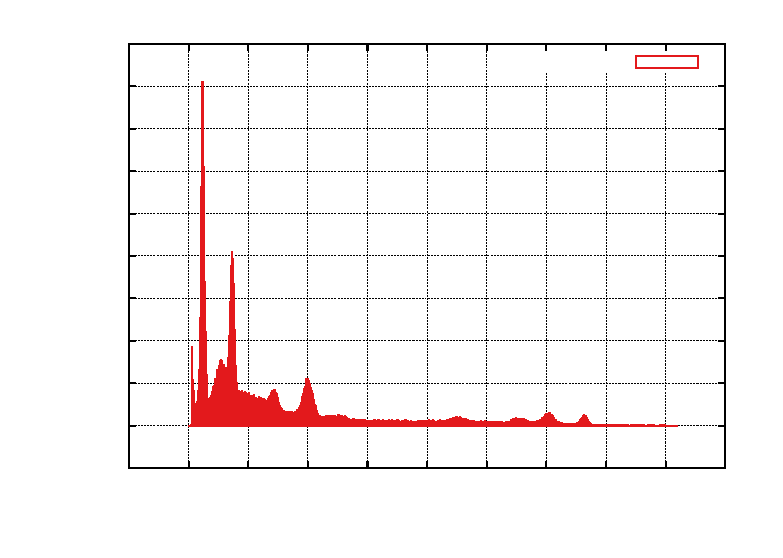
\includegraphics{./plots/szintillator/europium}}%
    \gplfronttext
  \end{picture}%
\endgroup

	\caption{Euroooopium szinti}
	\label{fig:europium_spektrum}
\end{figure}

\begin{figure}[h]
	\centering
	% GNUPLOT: LaTeX picture with Postscript
\begingroup
  \makeatletter
  \providecommand\color[2][]{%
    \GenericError{(gnuplot) \space\space\space\@spaces}{%
      Package color not loaded in conjunction with
      terminal option `colourtext'%
    }{See the gnuplot documentation for explanation.%
    }{Either use 'blacktext' in gnuplot or load the package
      color.sty in LaTeX.}%
    \renewcommand\color[2][]{}%
  }%
  \providecommand\includegraphics[2][]{%
    \GenericError{(gnuplot) \space\space\space\@spaces}{%
      Package graphicx or graphics not loaded%
    }{See the gnuplot documentation for explanation.%
    }{The gnuplot epslatex terminal needs graphicx.sty or graphics.sty.}%
    \renewcommand\includegraphics[2][]{}%
  }%
  \providecommand\rotatebox[2]{#2}%
  \@ifundefined{ifGPcolor}{%
    \newif\ifGPcolor
    \GPcolortrue
  }{}%
  \@ifundefined{ifGPblacktext}{%
    \newif\ifGPblacktext
    \GPblacktexttrue
  }{}%
  % define a \g@addto@macro without @ in the name:
  \let\gplgaddtomacro\g@addto@macro
  % define empty templates for all commands taking text:
  \gdef\gplbacktext{}%
  \gdef\gplfronttext{}%
  \makeatother
  \ifGPblacktext
    % no textcolor at all
    \def\colorrgb#1{}%
    \def\colorgray#1{}%
  \else
    % gray or color?
    \ifGPcolor
      \def\colorrgb#1{\color[rgb]{#1}}%
      \def\colorgray#1{\color[gray]{#1}}%
      \expandafter\def\csname LTw\endcsname{\color{white}}%
      \expandafter\def\csname LTb\endcsname{\color{black}}%
      \expandafter\def\csname LTa\endcsname{\color{black}}%
      \expandafter\def\csname LT0\endcsname{\color[rgb]{1,0,0}}%
      \expandafter\def\csname LT1\endcsname{\color[rgb]{0,1,0}}%
      \expandafter\def\csname LT2\endcsname{\color[rgb]{0,0,1}}%
      \expandafter\def\csname LT3\endcsname{\color[rgb]{1,0,1}}%
      \expandafter\def\csname LT4\endcsname{\color[rgb]{0,1,1}}%
      \expandafter\def\csname LT5\endcsname{\color[rgb]{1,1,0}}%
      \expandafter\def\csname LT6\endcsname{\color[rgb]{0,0,0}}%
      \expandafter\def\csname LT7\endcsname{\color[rgb]{1,0.3,0}}%
      \expandafter\def\csname LT8\endcsname{\color[rgb]{0.5,0.5,0.5}}%
    \else
      % gray
      \def\colorrgb#1{\color{black}}%
      \def\colorgray#1{\color[gray]{#1}}%
      \expandafter\def\csname LTw\endcsname{\color{white}}%
      \expandafter\def\csname LTb\endcsname{\color{black}}%
      \expandafter\def\csname LTa\endcsname{\color{black}}%
      \expandafter\def\csname LT0\endcsname{\color{black}}%
      \expandafter\def\csname LT1\endcsname{\color{black}}%
      \expandafter\def\csname LT2\endcsname{\color{black}}%
      \expandafter\def\csname LT3\endcsname{\color{black}}%
      \expandafter\def\csname LT4\endcsname{\color{black}}%
      \expandafter\def\csname LT5\endcsname{\color{black}}%
      \expandafter\def\csname LT6\endcsname{\color{black}}%
      \expandafter\def\csname LT7\endcsname{\color{black}}%
      \expandafter\def\csname LT8\endcsname{\color{black}}%
    \fi
  \fi
    \setlength{\unitlength}{0.0500bp}%
    \ifx\gptboxheight\undefined%
      \newlength{\gptboxheight}%
      \newlength{\gptboxwidth}%
      \newsavebox{\gptboxtext}%
    \fi%
    \setlength{\fboxrule}{0.5pt}%
    \setlength{\fboxsep}{1pt}%
\begin{picture}(7200.00,5040.00)%
    \gplgaddtomacro\gplbacktext{%
      \csname LTb\endcsname%
      \put(946,704){\makebox(0,0)[r]{\strut{}$0$}}%
      \csname LTb\endcsname%
      \put(946,1286){\makebox(0,0)[r]{\strut{}$200$}}%
      \csname LTb\endcsname%
      \put(946,1867){\makebox(0,0)[r]{\strut{}$400$}}%
      \csname LTb\endcsname%
      \put(946,2449){\makebox(0,0)[r]{\strut{}$600$}}%
      \csname LTb\endcsname%
      \put(946,3030){\makebox(0,0)[r]{\strut{}$800$}}%
      \csname LTb\endcsname%
      \put(946,3612){\makebox(0,0)[r]{\strut{}$1000$}}%
      \csname LTb\endcsname%
      \put(946,4193){\makebox(0,0)[r]{\strut{}$1200$}}%
      \csname LTb\endcsname%
      \put(946,4775){\makebox(0,0)[r]{\strut{}$1400$}}%
      \csname LTb\endcsname%
      \put(1078,484){\makebox(0,0){\strut{}$0$}}%
      \csname LTb\endcsname%
      \put(2223,484){\makebox(0,0){\strut{}$1000$}}%
      \csname LTb\endcsname%
      \put(3368,484){\makebox(0,0){\strut{}$2000$}}%
      \csname LTb\endcsname%
      \put(4513,484){\makebox(0,0){\strut{}$3000$}}%
      \csname LTb\endcsname%
      \put(5658,484){\makebox(0,0){\strut{}$4000$}}%
      \csname LTb\endcsname%
      \put(6803,484){\makebox(0,0){\strut{}$5000$}}%
    }%
    \gplgaddtomacro\gplfronttext{%
      \csname LTb\endcsname%
      \put(176,2739){\rotatebox{-270}{\makebox(0,0){\strut{}Ereignisse $N$}}}%
      \put(3940,154){\makebox(0,0){\strut{}Kanal $n$}}%
      \csname LTb\endcsname%
      \put(5816,4602){\makebox(0,0)[r]{\strut{}Messwerte}}%
    }%
    \gplbacktext
    \put(0,0){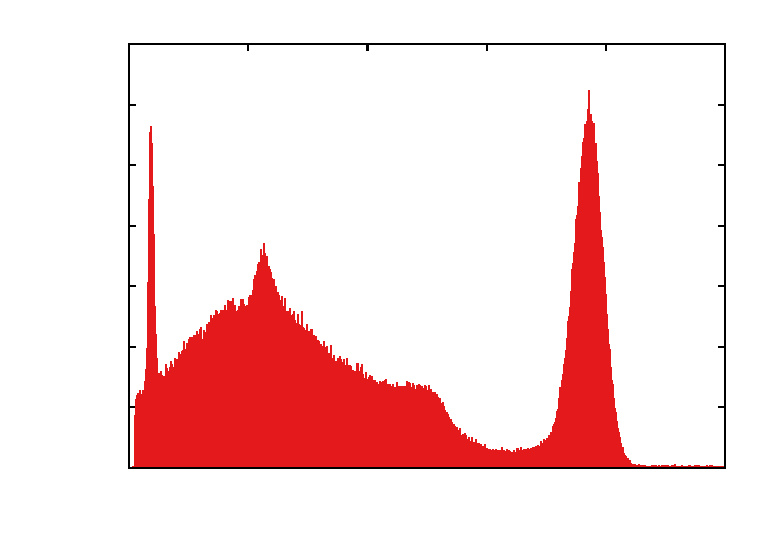
\includegraphics{./plots/szintillator/caesium}}%
    \gplfronttext
  \end{picture}%
\endgroup

	\caption{Cääääääsium halbleiter}
	\label{fig:caesium_spektrum}
\end{figure}

\begin{figure}[h]
	\centering
	% GNUPLOT: LaTeX picture with Postscript
\begingroup
  \makeatletter
  \providecommand\color[2][]{%
    \GenericError{(gnuplot) \space\space\space\@spaces}{%
      Package color not loaded in conjunction with
      terminal option `colourtext'%
    }{See the gnuplot documentation for explanation.%
    }{Either use 'blacktext' in gnuplot or load the package
      color.sty in LaTeX.}%
    \renewcommand\color[2][]{}%
  }%
  \providecommand\includegraphics[2][]{%
    \GenericError{(gnuplot) \space\space\space\@spaces}{%
      Package graphicx or graphics not loaded%
    }{See the gnuplot documentation for explanation.%
    }{The gnuplot epslatex terminal needs graphicx.sty or graphics.sty.}%
    \renewcommand\includegraphics[2][]{}%
  }%
  \providecommand\rotatebox[2]{#2}%
  \@ifundefined{ifGPcolor}{%
    \newif\ifGPcolor
    \GPcolortrue
  }{}%
  \@ifundefined{ifGPblacktext}{%
    \newif\ifGPblacktext
    \GPblacktexttrue
  }{}%
  % define a \g@addto@macro without @ in the name:
  \let\gplgaddtomacro\g@addto@macro
  % define empty templates for all commands taking text:
  \gdef\gplbacktext{}%
  \gdef\gplfronttext{}%
  \makeatother
  \ifGPblacktext
    % no textcolor at all
    \def\colorrgb#1{}%
    \def\colorgray#1{}%
  \else
    % gray or color?
    \ifGPcolor
      \def\colorrgb#1{\color[rgb]{#1}}%
      \def\colorgray#1{\color[gray]{#1}}%
      \expandafter\def\csname LTw\endcsname{\color{white}}%
      \expandafter\def\csname LTb\endcsname{\color{black}}%
      \expandafter\def\csname LTa\endcsname{\color{black}}%
      \expandafter\def\csname LT0\endcsname{\color[rgb]{1,0,0}}%
      \expandafter\def\csname LT1\endcsname{\color[rgb]{0,1,0}}%
      \expandafter\def\csname LT2\endcsname{\color[rgb]{0,0,1}}%
      \expandafter\def\csname LT3\endcsname{\color[rgb]{1,0,1}}%
      \expandafter\def\csname LT4\endcsname{\color[rgb]{0,1,1}}%
      \expandafter\def\csname LT5\endcsname{\color[rgb]{1,1,0}}%
      \expandafter\def\csname LT6\endcsname{\color[rgb]{0,0,0}}%
      \expandafter\def\csname LT7\endcsname{\color[rgb]{1,0.3,0}}%
      \expandafter\def\csname LT8\endcsname{\color[rgb]{0.5,0.5,0.5}}%
    \else
      % gray
      \def\colorrgb#1{\color{black}}%
      \def\colorgray#1{\color[gray]{#1}}%
      \expandafter\def\csname LTw\endcsname{\color{white}}%
      \expandafter\def\csname LTb\endcsname{\color{black}}%
      \expandafter\def\csname LTa\endcsname{\color{black}}%
      \expandafter\def\csname LT0\endcsname{\color{black}}%
      \expandafter\def\csname LT1\endcsname{\color{black}}%
      \expandafter\def\csname LT2\endcsname{\color{black}}%
      \expandafter\def\csname LT3\endcsname{\color{black}}%
      \expandafter\def\csname LT4\endcsname{\color{black}}%
      \expandafter\def\csname LT5\endcsname{\color{black}}%
      \expandafter\def\csname LT6\endcsname{\color{black}}%
      \expandafter\def\csname LT7\endcsname{\color{black}}%
      \expandafter\def\csname LT8\endcsname{\color{black}}%
    \fi
  \fi
    \setlength{\unitlength}{0.0500bp}%
    \ifx\gptboxheight\undefined%
      \newlength{\gptboxheight}%
      \newlength{\gptboxwidth}%
      \newsavebox{\gptboxtext}%
    \fi%
    \setlength{\fboxrule}{0.5pt}%
    \setlength{\fboxsep}{1pt}%
\begin{picture}(7200.00,5040.00)%
    \gplgaddtomacro\gplbacktext{%
      \csname LTb\endcsname%
      \put(1078,704){\makebox(0,0)[r]{\strut{}$0$}}%
      \csname LTb\endcsname%
      \put(1078,1383){\makebox(0,0)[r]{\strut{}$2000$}}%
      \csname LTb\endcsname%
      \put(1078,2061){\makebox(0,0)[r]{\strut{}$4000$}}%
      \csname LTb\endcsname%
      \put(1078,2740){\makebox(0,0)[r]{\strut{}$6000$}}%
      \csname LTb\endcsname%
      \put(1078,3418){\makebox(0,0)[r]{\strut{}$8000$}}%
      \csname LTb\endcsname%
      \put(1078,4097){\makebox(0,0)[r]{\strut{}$10000$}}%
      \csname LTb\endcsname%
      \put(1078,4775){\makebox(0,0)[r]{\strut{}$12000$}}%
      \csname LTb\endcsname%
      \put(1210,484){\makebox(0,0){\strut{}$0$}}%
      \csname LTb\endcsname%
      \put(1831,484){\makebox(0,0){\strut{}$1000$}}%
      \csname LTb\endcsname%
      \put(2453,484){\makebox(0,0){\strut{}$2000$}}%
      \csname LTb\endcsname%
      \put(3074,484){\makebox(0,0){\strut{}$3000$}}%
      \csname LTb\endcsname%
      \put(3696,484){\makebox(0,0){\strut{}$4000$}}%
      \csname LTb\endcsname%
      \put(4317,484){\makebox(0,0){\strut{}$5000$}}%
      \csname LTb\endcsname%
      \put(4939,484){\makebox(0,0){\strut{}$6000$}}%
      \csname LTb\endcsname%
      \put(5560,484){\makebox(0,0){\strut{}$7000$}}%
      \csname LTb\endcsname%
      \put(6182,484){\makebox(0,0){\strut{}$8000$}}%
      \csname LTb\endcsname%
      \put(6803,484){\makebox(0,0){\strut{}$9000$}}%
    }%
    \gplgaddtomacro\gplfronttext{%
      \csname LTb\endcsname%
      \put(176,2739){\rotatebox{-270}{\makebox(0,0){\strut{}Ereignisse $$}}}%
      \put(4006,154){\makebox(0,0){\strut{}Kanal $n$}}%
      \csname LTb\endcsname%
      \put(2530,4602){\makebox(0,0)[r]{\strut{}Messwerte}}%
    }%
    \gplbacktext
    \put(0,0){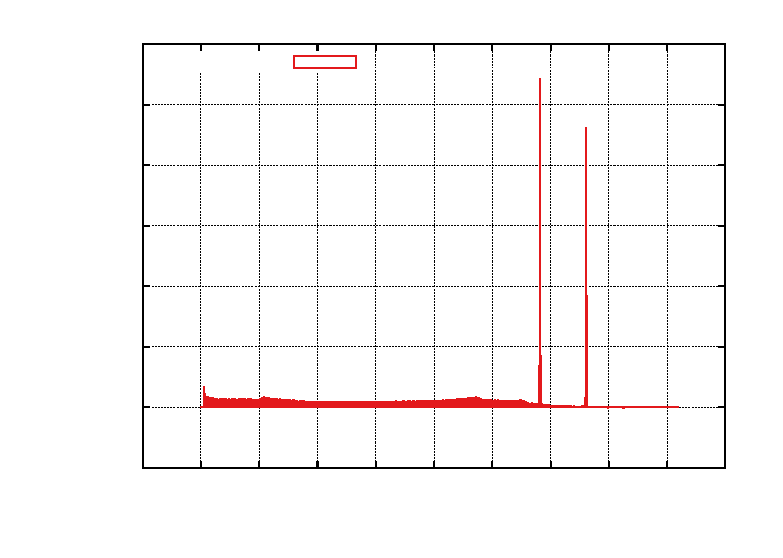
\includegraphics{./plots/halbleiter/cobalt}}%
    \gplfronttext
  \end{picture}%
\endgroup

	\caption{Cooooobalt halbleiter}
	\label{fig:cobalt_spektrum}
\end{figure}

\begin{figure}[h]
	\centering
	% GNUPLOT: LaTeX picture with Postscript
\begingroup
  \makeatletter
  \providecommand\color[2][]{%
    \GenericError{(gnuplot) \space\space\space\@spaces}{%
      Package color not loaded in conjunction with
      terminal option `colourtext'%
    }{See the gnuplot documentation for explanation.%
    }{Either use 'blacktext' in gnuplot or load the package
      color.sty in LaTeX.}%
    \renewcommand\color[2][]{}%
  }%
  \providecommand\includegraphics[2][]{%
    \GenericError{(gnuplot) \space\space\space\@spaces}{%
      Package graphicx or graphics not loaded%
    }{See the gnuplot documentation for explanation.%
    }{The gnuplot epslatex terminal needs graphicx.sty or graphics.sty.}%
    \renewcommand\includegraphics[2][]{}%
  }%
  \providecommand\rotatebox[2]{#2}%
  \@ifundefined{ifGPcolor}{%
    \newif\ifGPcolor
    \GPcolortrue
  }{}%
  \@ifundefined{ifGPblacktext}{%
    \newif\ifGPblacktext
    \GPblacktexttrue
  }{}%
  % define a \g@addto@macro without @ in the name:
  \let\gplgaddtomacro\g@addto@macro
  % define empty templates for all commands taking text:
  \gdef\gplbacktext{}%
  \gdef\gplfronttext{}%
  \makeatother
  \ifGPblacktext
    % no textcolor at all
    \def\colorrgb#1{}%
    \def\colorgray#1{}%
  \else
    % gray or color?
    \ifGPcolor
      \def\colorrgb#1{\color[rgb]{#1}}%
      \def\colorgray#1{\color[gray]{#1}}%
      \expandafter\def\csname LTw\endcsname{\color{white}}%
      \expandafter\def\csname LTb\endcsname{\color{black}}%
      \expandafter\def\csname LTa\endcsname{\color{black}}%
      \expandafter\def\csname LT0\endcsname{\color[rgb]{1,0,0}}%
      \expandafter\def\csname LT1\endcsname{\color[rgb]{0,1,0}}%
      \expandafter\def\csname LT2\endcsname{\color[rgb]{0,0,1}}%
      \expandafter\def\csname LT3\endcsname{\color[rgb]{1,0,1}}%
      \expandafter\def\csname LT4\endcsname{\color[rgb]{0,1,1}}%
      \expandafter\def\csname LT5\endcsname{\color[rgb]{1,1,0}}%
      \expandafter\def\csname LT6\endcsname{\color[rgb]{0,0,0}}%
      \expandafter\def\csname LT7\endcsname{\color[rgb]{1,0.3,0}}%
      \expandafter\def\csname LT8\endcsname{\color[rgb]{0.5,0.5,0.5}}%
    \else
      % gray
      \def\colorrgb#1{\color{black}}%
      \def\colorgray#1{\color[gray]{#1}}%
      \expandafter\def\csname LTw\endcsname{\color{white}}%
      \expandafter\def\csname LTb\endcsname{\color{black}}%
      \expandafter\def\csname LTa\endcsname{\color{black}}%
      \expandafter\def\csname LT0\endcsname{\color{black}}%
      \expandafter\def\csname LT1\endcsname{\color{black}}%
      \expandafter\def\csname LT2\endcsname{\color{black}}%
      \expandafter\def\csname LT3\endcsname{\color{black}}%
      \expandafter\def\csname LT4\endcsname{\color{black}}%
      \expandafter\def\csname LT5\endcsname{\color{black}}%
      \expandafter\def\csname LT6\endcsname{\color{black}}%
      \expandafter\def\csname LT7\endcsname{\color{black}}%
      \expandafter\def\csname LT8\endcsname{\color{black}}%
    \fi
  \fi
    \setlength{\unitlength}{0.0500bp}%
    \ifx\gptboxheight\undefined%
      \newlength{\gptboxheight}%
      \newlength{\gptboxwidth}%
      \newsavebox{\gptboxtext}%
    \fi%
    \setlength{\fboxrule}{0.5pt}%
    \setlength{\fboxsep}{1pt}%
\begin{picture}(7200.00,5040.00)%
    \gplgaddtomacro\gplbacktext{%
      \csname LTb\endcsname%
      \put(946,704){\makebox(0,0)[r]{\strut{}$0$}}%
      \put(946,1156){\makebox(0,0)[r]{\strut{}$500$}}%
      \put(946,1609){\makebox(0,0)[r]{\strut{}$1000$}}%
      \put(946,2061){\makebox(0,0)[r]{\strut{}$1500$}}%
      \put(946,2513){\makebox(0,0)[r]{\strut{}$2000$}}%
      \put(946,2966){\makebox(0,0)[r]{\strut{}$2500$}}%
      \put(946,3418){\makebox(0,0)[r]{\strut{}$3000$}}%
      \put(946,3870){\makebox(0,0)[r]{\strut{}$3500$}}%
      \put(946,4323){\makebox(0,0)[r]{\strut{}$4000$}}%
      \put(946,4775){\makebox(0,0)[r]{\strut{}$4500$}}%
      \put(1078,484){\makebox(0,0){\strut{}$0$}}%
      \put(1896,484){\makebox(0,0){\strut{}$1000$}}%
      \put(2714,484){\makebox(0,0){\strut{}$2000$}}%
      \put(3532,484){\makebox(0,0){\strut{}$3000$}}%
      \put(4349,484){\makebox(0,0){\strut{}$4000$}}%
      \put(5167,484){\makebox(0,0){\strut{}$5000$}}%
      \put(5985,484){\makebox(0,0){\strut{}$6000$}}%
      \put(6803,484){\makebox(0,0){\strut{}$7000$}}%
      \put(1413,3508){\rotatebox{-270}{\makebox(0,0)[l]{\strut{}Röntgenlinie}}}%
      \put(1675,2716){\rotatebox{-270}{\makebox(0,0)[l]{\strut{}\SI{121.783}{keV}}}}%
      \put(2256,1240){\rotatebox{-270}{\makebox(0,0)[l]{\strut{}\SI{244.699}{keV}}}}%
      \put(2706,1315){\rotatebox{-270}{\makebox(0,0)[l]{\strut{}\SI{344.281}{keV}}}}%
      \put(4769,930){\rotatebox{-270}{\makebox(0,0)[l]{\strut{}\SI{778.903}{keV}}}}%
      \put(5599,921){\rotatebox{-270}{\makebox(0,0)[l]{\strut{}\SI{964.131}{keV}}}}%
      \put(6006,995){\rotatebox{-270}{\makebox(0,0)[l]{\strut{}\SI{1112.116}{keV}}}}%
      \put(6492,948){\rotatebox{-270}{\makebox(0,0)[l]{\strut{}\SI{1408.011}{keV}}}}%
    }%
    \gplgaddtomacro\gplfronttext{%
      \csname LTb\endcsname%
      \put(176,2739){\rotatebox{-270}{\makebox(0,0){\strut{}Ereignisse $N$}}}%
      \put(3940,154){\makebox(0,0){\strut{}Kanal $n$}}%
    }%
    \gplbacktext
    \put(0,0){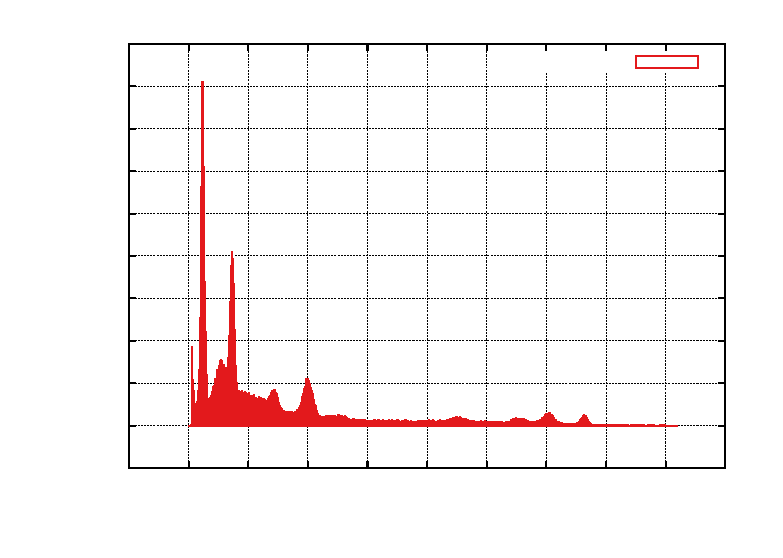
\includegraphics{./plots/szintillator/europium}}%
    \gplfronttext
  \end{picture}%
\endgroup

	\caption{Euroooopium halbleiter}
	\label{fig:europium_spektrum}
\end{figure}

\subsection{Spektrum, Vielkanalanalysator}

\subsection{Auflösungsvermögen, Breite, Unterschiede der Detektoren}

\subsection{Nachweiswahrscheinlichkeit}

\subsection{Termschemata}


\section{Versuchsaufbau}

\section{Durchführung und Auswertung}
Die ausführliche Durchführung ist der Versuchsanleitung \cite{anleitung} zu entnehmen.
Sollten Abweichungen bei der Durchführung auftreten, so werden diese im jeweiligen Unterkapitel dargestellt.
\\
\\
Wenn nicht anders angegeben sind die dargestellten und genutzten Messwerte bereits um den Untergrund bereinigt worden.

\subsection{NaJ(Tl) Szintillationsspektrometer}

\subsubsection{Detektorsignal des Szintillationsdetektors}
\begin{figure}[h]
	\centering
	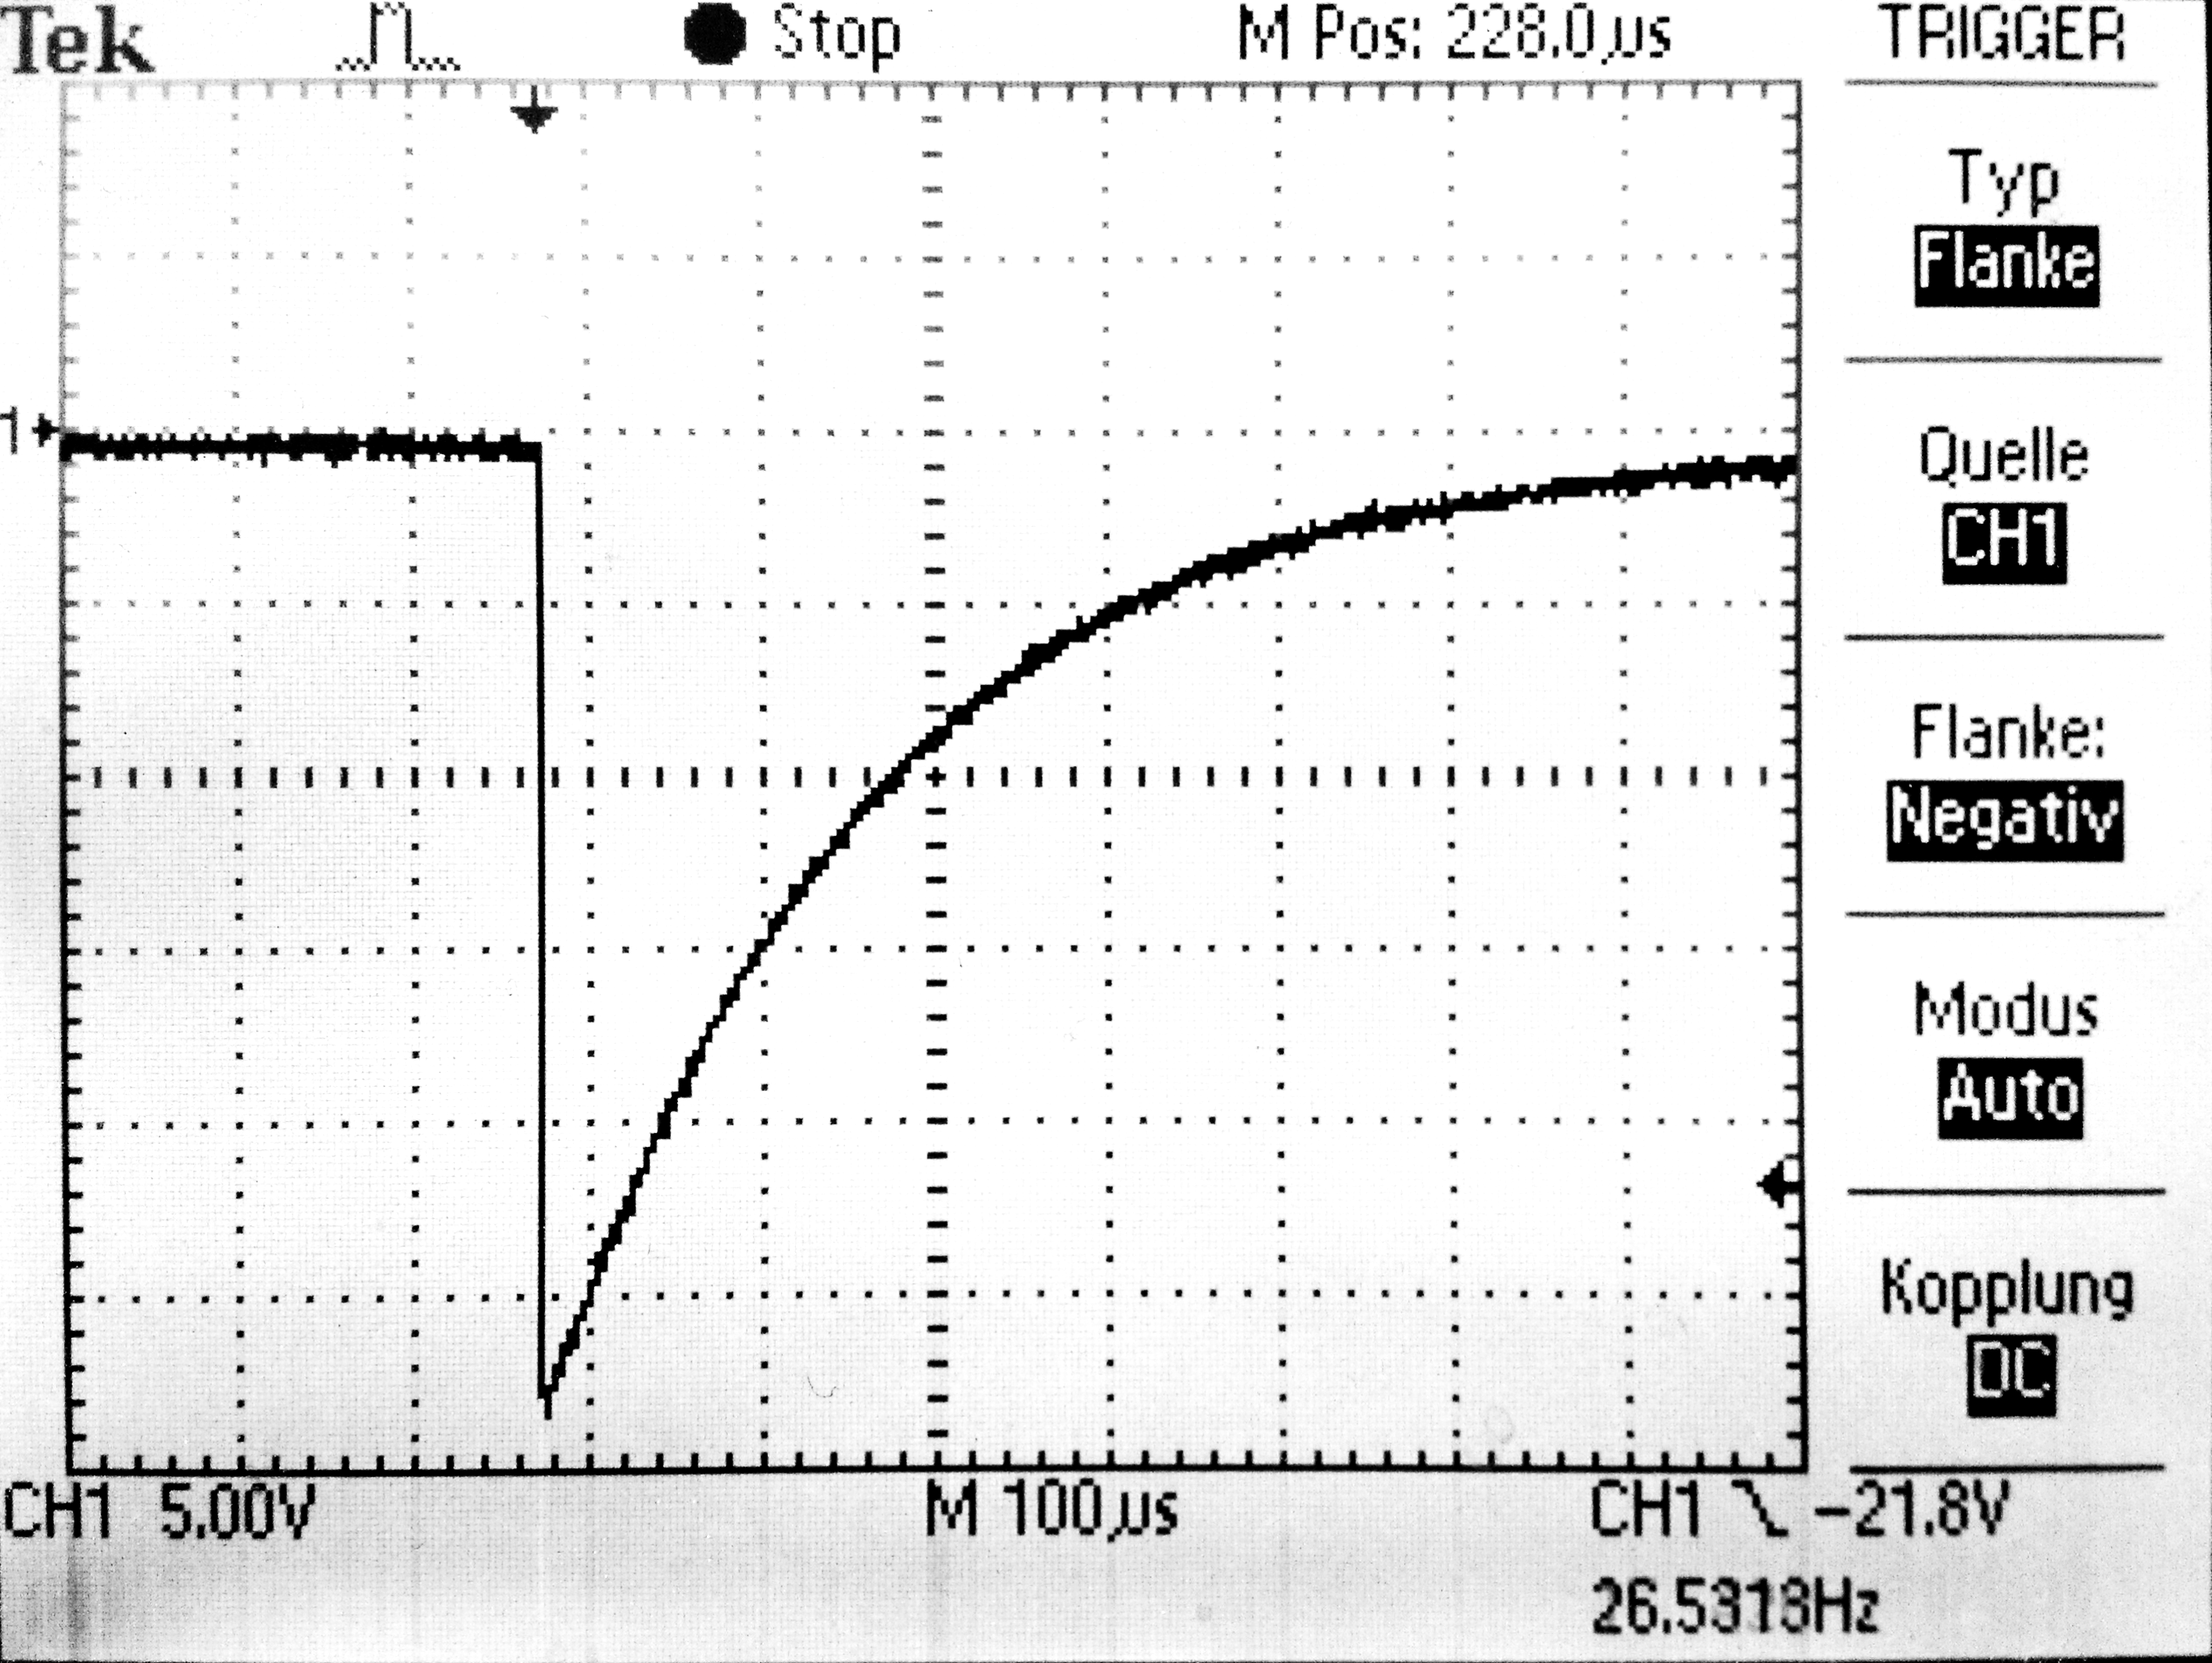
\includegraphics[width=
	0.7\textwidth]{./figures/signale/vor_szinti.png}
	\caption{Signal am Vorverstärker des Szintillators}
	\label{fig:signal_szinti_vor}
\end{figure}
\begin{figure}[h]
	\centering
	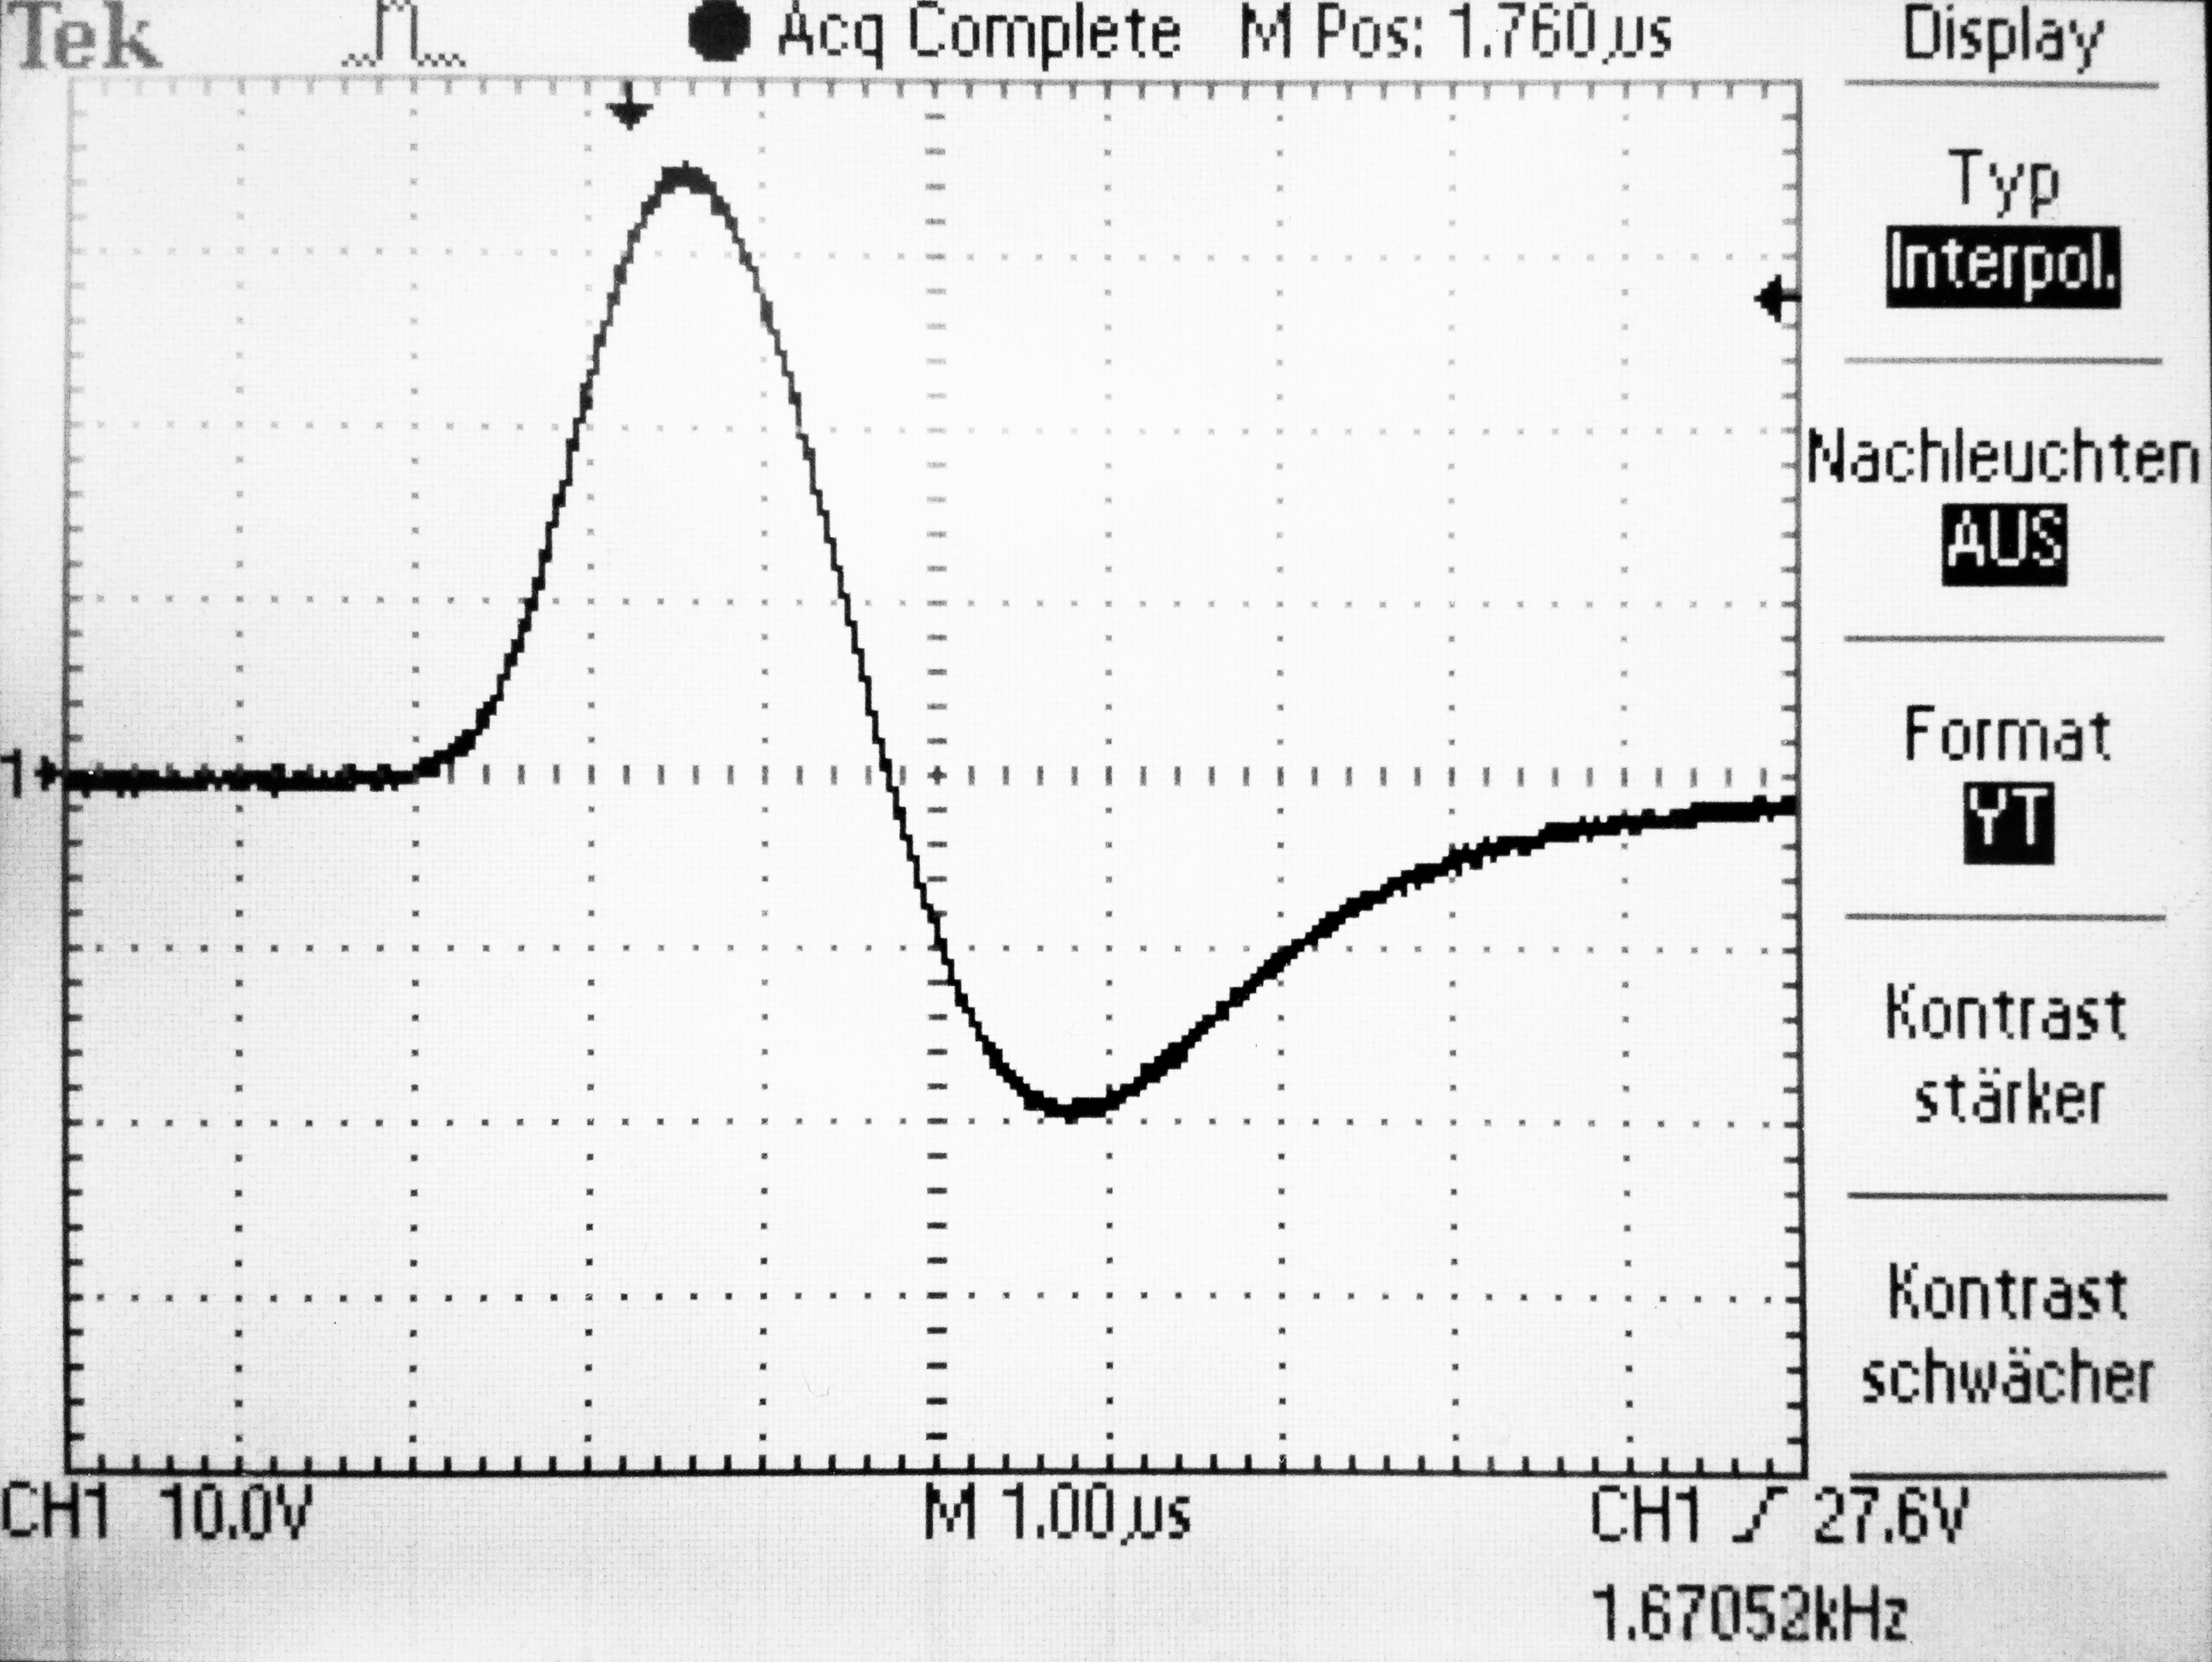
\includegraphics[width=0.7\textwidth]{./figures/signale/haupt_szinti.png}
	\caption{Signal am Hauptverstärker des Szintillators}
	\label{fig:signal_szinti_haupt}
\end{figure}
(KANNST DU DAS MENÜ RECHTS ABSCHNEIDEN? DAS CH1... xyz V soundso kHz kann auch weg aber rechts die x und y divisions nicht wegmachen)

\subsubsection{Aufnahme der Gammaspektren (QUELLEN) und das Untergrundspektrum}

\subsubsection{Energiekalibrierung}

\subsubsection{Halbwertsbreiten der Linien}

\subsubsection{Peak-to-Total Verhältnis}

\subsubsection{Absolute Peakeffizienz}



\subsection{Germanium Halbleiterdetektor}

\subsubsection{Detektorsignal des Szintillationsdetektors}

\subsubsection{Aufnahme der Gammaspektren (QUELLEN) und des Untergrundspektrums}

\subsubsection{Energiekalibrierung}

\subsubsection{Bestimmung der Halbwertsbreite}

\subsubsection{Intrinsische Halbwertsbreite}

\subsubsection{Peak-to-Total-Verhältnis}

\subsubsection{Absolute Peakeffizienz}

\subsubsection{Relative Effizienz als Funktion der Gammaenergie}

\subsection{Nachweis der Radioakivität in einer Probe}

\section{Fazit}

\FloatBarrier
% BIBLIOGRAPHIE
\vspace{\fill}
% Maximale Anzahl der Einträge in Klammer
% Zitieren mit \cite{lamport94}
\begin{thebibliography}{19}

\bibitem{krane}

\bibitem{siegbahn}
	K. Siegbahn,
	\emph{Alpha-, Beta- and Gamma-Ray Spectroscopy},
	Elsevier Science Ltd. 1965

\bibitem{anleitung}
	Physikalisches Praktikum V: Kern- und Teilchenphysik,
	Versuchsbeschreibung \emph{P523: $\beta$-Spektrometer} (Stand: Januar 2015),
	Universität Bonn	

\bibitem{riezler}
	Riezler, W.; Kopitzki, K.
	\emph{Kernphysikalisches Praktikum},
	Teubner 1963

\end{thebibliography}

% APPENDIX
\begin{appendix}
\section{Anhang}
Auf den folgenden Seiten sind der Vollständigkeit halber alle gemessenen Werte sowie die jeweils zur Auswertung berechneten Werte zusammengetragen.
\clearpage

\end{appendix}

\end{document}
